% This \addtocontents{...} magic is to move the chapter title to the 
% next page in the ToC to keep it with the subsections
% https://tex.stackexchange.com/questions/106289/keep-chapter-headings-and-related-subheadings-in-the-same-page-in-toc
\addtocontents{toc}{\newpage}
\chapter{Validation of Application Energy Monitoring}
\label{chapter:validation}

%%
%% TODO
%%
%% Possible additional testing:
%%   - Run multiple service type tests (e.g. mixed data and CPU)
%%   - Run multiple service instance tests (e.g. two CPU Hogs)
%%   - Run multiple machine tests
%%

\section{Introduction}

As described in \cref{chapter:implementation} we have implemented a proof-of-concept version of the Apollo energy allocation system, to prove the usefulness of our approach for allocating the energy consumed by underlying host systems to individual application requests executing on them.  The software was tested during development to ensure correctness with respect to expected results through unit and integration tests but now needs to be validated by using it in realistic test cases.  This process is described in this chapter.

In order to validate Apollo with realistic test cases, we need to define the kind of validation we are interested in achieving.  There are four validation goals that we wish to achieve, as listed below.

\begin{description}
\item [Validation Goal 1] We need to validate the \emph{calculation correctness} of Apollo's results, by running the calculator in one or more controlled scenarios where we can also gather additional runtime statistics that allow a separate independent calculation of a fair energy consumption and manually perform these calculations and use them to check the correctness of Apollo's results in the same scenarios.

\item [Validation Goal 2] We also need to validate the \emph{calculation consistency} of Apollo's results across a range of scenarios, to ensure that the same result is calculated consistently for equivalent but different workloads (e.g. 5 tasks of 1 CPU second workload produce the same result as 1 task containing 5 CPU seconds of workload, when all other factors remain constant).

\item [Validation Goal 3] We need to validate the \emph{energy allocation algorithm} when an application scenario is run on a host machine with different amounts of competing workload.  Specifically, as competing workload on a machine rises and other factors are held constant, the energy allocation for an application scenario should fall, to reflect it's declining proportional usage of the machine.

\item [Validation Goal 4] We want to validate \emph{CPU usage as a proxy for resource usage} when performing energy allocation calculations.  For this validation, we focus on how CPU usage varies for disk IO intensive workloads.

\end{description}

Throughout this validation testing, we aim to achieve consistency of results to within 5\% tolerance.  Long experience has taught us that a high degree of consistency is very difficult to achieve in any performance or resource utilisation testing due to the number of factors that can affect the results of a test on a modern multi-cpu, multi-core server machine.  Our experience in previous testing work is that a 5\% tolerance in most cases is the lowest degree of variation we are likely to achieve, being equivalent to equality plus the variation caused by factors outside our control.

\section{Testing Approach}

\subsection{The Test Application}

To allow us to test Apollo, we needed to reliably and reproducibly generate application workload that we could monitor, collect data for and run Apollo on the results.  We briefly considered using a real application such as an existing enterprise application or an open source business domain application.  However, it quickly became clear that using a real application would make the validation of the Apollo calculator almost impossible as it would be very difficult to make the application workload highly predictable and repeatable, to allow validation of the calculations performed.

Therefore, we decided to create a simple application, specifically designed to allow predictable application workloads to be generated and reproduced on demand.  The application contains four microservices implemented in Java:

\begin{itemize}
	\item A \emph{Gateway Service} that provides a simple entry point to the application for a benchmarking client to call and acts as an API gateway \cite{amundsen2016-uservices} for the application.  The Gateway Service contains configuration to define repeatable application scenarios that can be invoked by name and this service then calls the other microservices as required for a particular scenario.
	\item A \emph{CPU Hog Service} that will consume a specified amount of CPU time, specified by a URL parameter to its service call.  The service can consume CPU time constantly for a timed period (e.g. 5 seconds) or it can consume a specified number of milliseconds of CPU time before returning.  It times itself for a timed period using the system clock (via the \texttt{java.lang.System.currentTimeMillis()} method) and measures its CPU time using the Java JMX monitoring facilities.
	\item A \emph{Memory Hog Service} that will consume a specified number of megabytes of (heap) memory, then wait for a specified number of seconds before attempting to release the memory.  The amount of memory and holding period are specified as URL parameters to its service call.  Given the design of the Java Virtual Machine (JVM) care must be taken when using a program to consume and release memory reliably, as the combination of JVM garbage collection and virtualisation of memory access means that the operating system process often does not increase or decrease its memory usage predictably in response to Java code increasing or decreasing memory usage.  The service is useful though for applying increased memory pressure on the machine at specific times.
	\item A \emph{File IO Hog Service} that will perform a specified amount of file IO when its service entry point is called.  The amount of IO to perform is specified in megabytes as a URL parameter.  This service works in a very specific way, to avoid possible IO system optimisations reducing the real IO performed, while also avoiding unnecessary CPU consumption.  The problem we could have is that if we repeatedly write blocks of predictable data (e.g. blocks containing the same value throughout or repeating short data sequences repeatedly) then there is a danger that the IO subsystem will avoid performing some of the IO operations by performing some sort of write compression.  On the other hand, if we generate a large number of blocks of truly random data, this will involve quite a lot of CPU usage, which distorts the operation of the service and could make it CPU rather than IO intensive.  Therefore, the service generates a set of resusable random blocks of data when it starts up and selects a random sequence of these blocks, using a cheap pseudo-random number generator (\texttt{java.util.Random}) when writing a file.  This minimises CPU usage during the writing of the file, while also ensuring enough randomness to avoid obvious IO system optimisations.
 \end{itemize}

 These services were implemented using Java 1.8 and version 1.5.7 of the widely-used Spring Boot application framework (to provide application services such as HTTP request handling, configuration, database access abstraction and dependency injection).  This minimised the amount of application code that had to be written, allowing us to focus on the code needed to implement the core purpose of each service.  The microservices were organised into separate source trees, built using the Gradle build utility.

 Once developed, and unit and integration tested, the services were packaged into Docker containers to allow easy versioning, deployment and monitoring via the Docker runtime system, which was required by our proof-of-concept version of Apollo.

\subsection{The Test Software}

In order to reliably run a large number of validation tests for Apollo, the process needed to be automated so that the execution of the tests and collection of the results was standardised, efficient and reliable.  This involved a number of different types of automation and tools.

We started with a Linux server machine as the test environment.  The specification of the machine and the specific version of Linux are not very important, but we selected a 4 CPU machine with Intel Xeon 2.3GHz CPUs, 16GB of memory and 50GB of SSD storage running Ubuntu 16.4.04, one of the Ubuntu stable, long-term support releases.  This is a reasonably large machine, but we selected this specification as it is representative of the sort of mid-range server class machine that forms the backbone of the server fleet of many large organisations today.  Microservice systems often utilise many smaller machines, but we quickly realised that while the Apollo system runs equally well on many smaller machines (due to the features of the open source tools it uses) consistency, repeatability and control were going to be reduced when using a number of hosts.  Therefore it was decided to do most of the testing using a single host machine that had sufficient capacity to run all of our services without resource contention.

The \emph{machine configuration} was automated using the open source Ansible system configuration tool, with a number of custom configuration files (or "playbooks" as they are known in the Ansible ecosystem) and some custom shell scrips defining the basic system configuration needed for the test environment, including updating the operating system and installing security patches, creating users and installing public keys, installing basic tools like Python and Git, installing Docker, and setting up some basic security mechanisms.

Once the machine configuration was complete, \emph{application configuration} and \emph{service configuration} were both automated using the Docker Compose tool, which is part of the Docker toolset.  Docker Compose allows a group of cooperating services to be defined in terms of the Docker container images they utilise, the specific configuration that each service applies to the base image and the dependencies between the services (such as one service needing to call another).  We defined a single Docker Compose configuration that included the application services and the data collection services we needed to provide the data for Apollo (Zipkin, MySQL, Telegraf and InfluxDB as discussed in \sref{section:resusageofappworkload}).  This approach allowed a simple operating system script to be used to call Docker Compose with this configuration to reliably start or stop all of the services via a single command.

The process of \emph{running tests and collecting outputs} was automated using a range of operating system utilities and custom shell scripts.  The process can run one or more test scenarios, which were defined in the configuration of the Gateway Service as explained in the previous section.  The process of running a test scenario involved:
\begin{itemize}
	\item Clearing the MySQL and InfluxDB metrics databases so that the results of the test could easily be exported to files.
	\item Starting the \texttt{mpstat} and \texttt{pidstat} operating system utilities as "background" processes, logging their outputs to files, so that operating system and service process resource utilisation could be analysed after the test had executed.
	\item Invoking the Gateway Service to run the requested scenario (and in turn, it would call the other services as the scenario definition defined).
	\item Stopping the operating system utilities cleanly to terminate resource utilisation statistics collection at a defined point.
	\item Exporting the execution traces, host and application resource utilisation metrics and Docker network metadata from the MySQL and InfluxDB databases and Docker, into files that could be used to re-populate databases at a later point in time for Apollo to use.
	\item Exporting the host level resource utilisation statistics from the \texttt{sar} utility into a text file to allow host level resource utilisation to be analysed after the test had executed.
	\item Gathering all of the outputs of the test into a \texttt{tar} archive file for easy storage and transfer.
\end{itemize}

When a particular test scenario needed competing workload on the host machine, the \texttt{OpenSSL} package's \texttt{speed} command was used to generate load on one or more of the host's CPUs.  This was a scripted process, invoked manually before test cases that required predictable competing workload on the server host.

Once test cases were available, the output archive data files were transferred to local machines and a scripted process to \emph{run Apollo on the test scenario output} was executed. This cleared the local MySQL and InfluxDB databases, loaded the trace and resource utilisation data from the scenario into these databases, unpacked the other data files from the scenario archive, and ran Apollo on these data sets.  The output of the Apollo calculator was then inspected to analyse the characteristics of the scenario and the energy allocation that it had been allotted.


\section{Validation Goal 1 - Validating the Allocation Calculation}
\label{sec:validatingcalculation}

Our first validation goal is to ensure that the allocation calculation performed by Apollo can be reproduced by hand, following the algorithm presented in the previous chapter, with an acceptable level of consistency between the two approaches.

We chose one of the simpler standard scenarios that we had used during the testing process, the \texttt{simple-cpu-x50} scenario, which repeatedly makes short calls to the CPU intensive service.  We decided to use a scenario based on just two services, the Gateway service and the CPU intensive service, both running on a single machine.  This was to keep the manual calculation process tractable and avoid inconsistencies and mistakes complicating the process.  The Apollo calculation algorithm is simply a process of aggregating results from individual application elements and so we were confident that if the result of calculation for a small number of application services was correct then this would result in a correct calculation process for more complex cases that were simply aggregations of the lower level calculations.

To perform the calculation process, we decided to use a different set of metrics data sources from the set used by Apollo, to validate the approach to data collection as well as the implementation of the algorithm.  The set of data that the calculations were based on was:


\begin{itemize}
	\item the \emph{Zipkin traces} from the scenario being studied, as there was no credible alternative to this data;
	\item the \emph{Docker network configuration} for the Docker subsystem that the application elements were running within, to allow the IP address to container mapping to be retrieved, and again this was the only source of this information;
	\item a set of \texttt{pidstat(1)} metrics for the application, showing the CPU utilisation every second for the application processes;
	\item a set of \texttt{mpstat(1)} metrics for the host machine which allowed us to assess how much CPU was being used by the host during the duration of the test trace;
	\item the \emph{SPECPower benchmark results} for a representative server model, similar to the host in use; and
	\item the output of the \texttt{ps(1)} command from the host machine with all of the application elements running, to allow the process IDs for the application elements to be retrieved.
\end{itemize}

The important point about the data sources we used for this calculation is that the key data sources for resource utilisation metrics were different to those used by Apollo, to allow a broader degree of validation than a simple recalculation using identical data would have allowed.  While Apollo gets its resource utilisation metrics from the Docker subsystem's statistics mechanism (gathered via the Telegraf metrics server), for our calculations we used the metrics from mpstat(1) and pidstat(1) as explained above.

The first step was to inspect the Zipkin trace data to allow the start and end points of the request to be identified.  The Zipkin trace data had been saved from the execution of the test scenario and was loaded into a MySQL database to allow it to be queried easily.

The root traces were extracted from the Zipkin database, by selecting all of those rows in \texttt{zipkin\_spans} where the \texttt{trace\_id} column was the same as the \texttt{span\_id} column:

\lstset{language=SQL}
\begin{lstlisting}
	SELECt * FROM zipkin_spans WHERE id=trace_id
\end{lstlisting}


From the row returned, we extracted a trace ID of \texttt{5896569591426873811}, a start time of \texttt{1534185668229000} (nano seconds since the "Epoch", equating to 20180813T184108.229Z), and a duration of \texttt{126292740} (nano seconds - 126.292 seconds)	which imply an end time of \texttt{1534185794521740} (being equivalent to 20180813T184314.522Z).

Using the trace ID we could then run a more complex query to extract the trace's spans and their attributes from the Zipkin database:

\lstset{language=SQL}
\begin{lstlisting}
	SELECT hex(s.trace_id) as trace_id, hex(s.id) as span_id,
	       hex(s.parent_id) as parent_id,
	       start_ts as start_time_usec, 
	       start_ts+duration as end_time_usec,
	       inet_ntoa(endpoint_ipv4 & conv("ffffffff", 16, 10)) as ipv4_address,
	       endpoint_port
	FROM zipkin_spans s, zipkin_annotations a
	WHERE s.trace_id = 5896569591426873811
	AND s.trace_id = a.trace_id
	AND s.id = a.span_id
	AND a_key = 'sr'
	ORDER BY start_ts
\end{lstlisting}

This allowed us to identify the spans making up the processing of the request and the IP addresses of the two application elements that handled the invocations as being \texttt{172.18.0.7} and \texttt{172.18.0.8}, which were the IP addresses of the Docker containers containing the microservices involved in handling the request.

The next step was a simple lookup of the IP addresses in the Docker network configuration which resulted in the container IDs of the two Docker containers that our application elements ran within.  The short form IDs returned were \texttt{c42b3d3bf4b2} for the Gateway container and \texttt{b75d29577eb9} for the CPU intensive container.

Having the container IDs allowed us to reliably identify the Linux process IDs of the Java virtual machines running our application elements.  By using the \texttt{ps} output we saved during the test execution, we could use the container IDs to find the Docker container daemon  processes running the JVMs for our services, with CPU intensive service and the Gateway service.

Having the process IDs allowed us to inspect the \texttt{pidstat} output that we had collected during test execution.   This utility captured CPU percentage usage statistics for our processes every second during the test period.

For the CPU intensive service, we found that its average CPU consumption was 25.42\% with a very low standard deviation of 0.26 across the test set.

For the Gateway process, we found that its average CPU consumption was 0.3\% of the machine (although this did have a maximum of 0.75\% for short periods, leading to a standard deviation of 0.11 for the test set).

Therefore, we decided to use 25.75\% as the container CPU usage during the test period.

The next step in the process was to estimate the energy usage of the underlying host machine.  We collected \texttt{sar} and \texttt{mpstat} resource utilisation metrics for the machine during the test period to provide host CPU utilisation metrics.  The \texttt{sar} statistics were of less use as this utility collects statistics every minute and so we had a limited number of samples but it appeared to indicate a total machine CPU usage of about 25\% during the test period.

The \texttt{mpstat} statistics were more useful as they contained a metric measurement for CPU usage percentage per CPU every second during the test period.  When we analysed this dataset we found that the machine's utilisation was a very constant 27\% right through the test period, apart from one second (10 seconds into the test) when it jumped to 75\% usage and then back down to 27\% (for reasons we weren't able to identify).

The CPU usage percentage allowed us to estimate the energy consumption of the machine using a representative set of SPEC Power benchmark results for a similar server model.  The benchmark results were 102W at 20\% and 120W at 30\%.  Therefore interpolation resulted in the value $((120 - 102) \times (7/10)) + 102 = 12.6 + 102 = 114.6W$.  That is, the machine's power consumption during the test period was about 114 J/second.

Given that the test period was 126.30 seconds, this resulted in a power consumption value for the host machine of $126.30 \times 114 = 14473.98J$, which we rounded to 14474J.

Given the host CPU usage, the CPU usage of our containers and the host power consumption we could now calculate the power allocation to our application trace.

Given a test length of 126.3 seconds and a 4 CPU host machine this means a total possible CPU resource available of:

\begin{equation}
126.3 \times 4 = 505.2 ~CPU seconds
\end{equation}

Our test data indicates that the host was busy for 27\% of the time during the test execution, therefore our total host CPU time consumed during the test period was:

\begin{equation}
505.2 \times 0.27 = 136.40 ~CPU seconds
\end{equation}

Our application processes (containers) consumed 25.75\% of the host's CPU time during the test period therefore their CPU usage is calculated as:

\begin{equation}
136.40 \times 0.2575 = 130.09 ~CPU seconds
\end{equation}

Given our CPU usage and the host energy consumption we can then calculate the energy allocation to our application request as being:

\begin{equation}
130.09 / 136.40 \times 14474 = 13804J
\end{equation}

We then ran the Apollo proof-of-concept implementation on the test scenario data set to compare our results, which are shown in \tref{table:calculationresults}

\begin{table}
\centering
\caption{Manual Calculation Compared to Apollo Calculation}
\label{table:calculationresults}
\footnotesize
\begin{tabular}{|c|c|c|c|}
\hline
Value & Manual Calculation & Apollo Calculation & Difference \\
\hline
\hline
Trace CPU msec       & 130090 & 124257 & 4.5\% \\
Host CPU msec        & 136404 & 132891 & 2.5\% \\
Host Energy J        & 14474  & 14213  & 1.8\% \\
Application Energy J & 13804  & 13290  & 3.9\% \\
\hline
\end{tabular}
\end{table}

As can be seen from the results in the table, using a manual calculation technique that attempts to mirror the algorithm used in Apollo, while using different data sources for the critical resource utilisation metrics, has resulted in a very close match between the results, with the manual calculation of the energy allocation for the application request trace being within 4\% of the automated Apollo value.

The difference in the results will be familiar to anyone who has been involved in performance testing, where repeatability of results is often very difficult to obtain (as evidenced by the subtle but constant inconsistencies in the numerical results from tools such as \texttt{sar}, \texttt{mpstat} and \texttt{pidstat}).  In our situation, as well as the normal difficulty of repeatability, we believe that most of the difference in these results is likely to be the result of Apollo using the finer grained Docker metrics, while the manual process relied on the coarser grained metrics from the standard system administration tools. 

This result is well within our target result tolerance and so validates the Apollo proof-of-concept implementation's accuracy and achieves validation goal 1.

\section{Validation Goal 2 - Validating Allocation Consistency}
\label{section:validatingconsistency}

Our second validation goal, is to validate consistency of energy allocation.  To achieve this, our strategy is to run a known control workload under fixed host utilisation conditions (no other workload being the simplest case) and to run a range of other workloads that we know contain an equivalent amount of computational work but are structured differently.  The energy allocation should be the same for each case.

In our first test, we structured a workload into three cases, each of which involved the same amount of CPU workload but in three different scenarios.  The first scenario invoked a short service call (involving 50msec of CPU work) 1000 times, the second scenario invoked a longer service call (500msec of CPU work) 100 times and the third ran a long service call (5000msec of CPU work) 10 times.  Each scenario was called 6 times to ensure a consistent result.

Our first question was whether the energy allocations per request were consistent across the three cases.  Our analysis of this question is shown in the scatter graph in \fref{figure:validation-energycpu}, which plots the energy usage against CPU workload for each of the scenarios executed, using logarithmic scales.

\begin{figure}
\centering
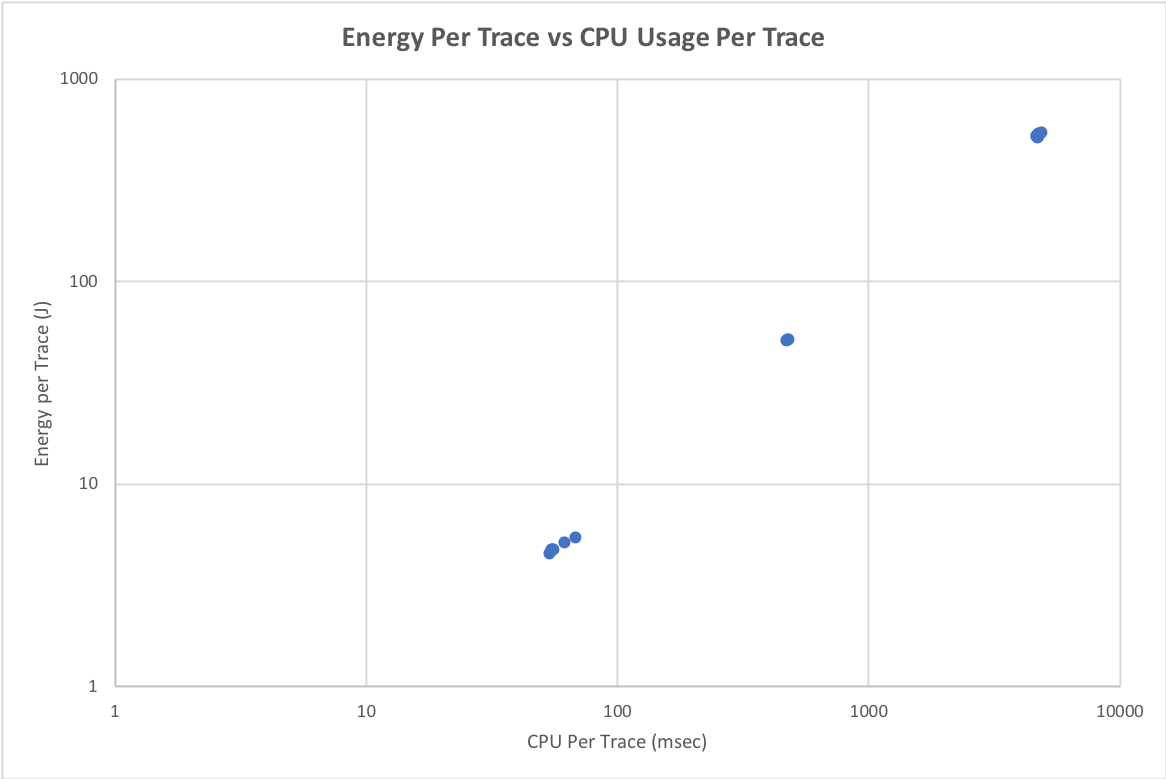
\includegraphics[width=0.75\textwidth,trim={3 3 3 3},clip]{Figures/validation-energycpu}
\caption{Energy Allocation per Request for Small, Medium and Large Services}
\label{figure:validation-energycpu}
\end{figure}

The graph shows the three sets of scenarios (short, medium and long) clearly clustering very closely, showing that the energy allocation per trace is extremely consistent across the three sets, suggesting that the allocation calculation is working consistently as designed.  More precisely, the correlation coefficient between the two sets of values is 0.999, indicating a very high degree of correlation between CPU consumed and energy allocation performed.

Our second test involved investigating how energy allocation was affected by a constant amount of CPU workload but in scenarios of different lengths.  To test this we repeatedly ran two scenarios, both of which contained the same amount of CPU workload (a trace that took 2,500 msec, run 50 times), with one scenario having pauses inserted into it, to cause the scenario to take longer to execute but consume no more CPU resource during the extended execution time.  In addition, for reasons which we explain below, we ran the first set of scenario tests with no additional load on the machine and the second set with synthetic workload consuming 50\% of the machine's CPU.  The results of this experiment are shown in the line graph in \fref{figure:validation-scenariolength}

\begin{figure}
\centering
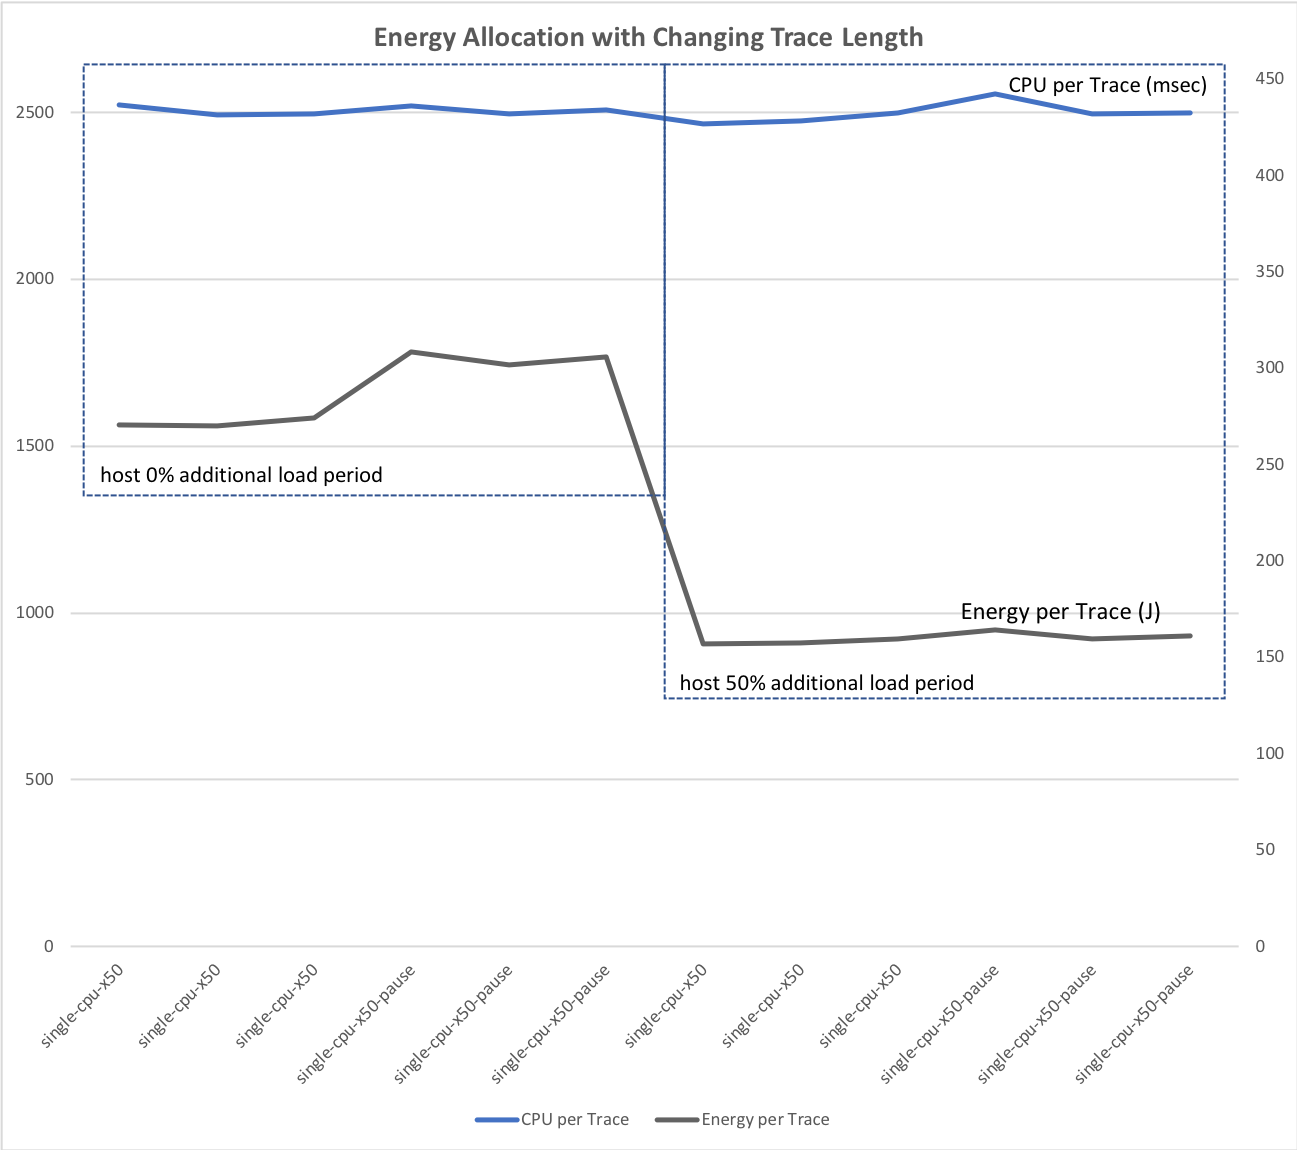
\includegraphics[width=0.75\textwidth,trim={2 2 2 2},clip]{Figures/validation-scenariolength}
\caption{Energy Allocation Across Different Scenario Lengths}
\label{figure:validation-scenariolength}
\end{figure}

This graph plots the CPU usage per trace (the top line) and the energy usage per trace (the bottom line) for sample executions of the scenarios.  As indicated by the dashed boxes annotating the graph, the first 6 executions were performed with no additional workload on the machine, the second 6 executions were performed with the machine having 50\% of its CPU capacity consumed by other synthetic workload.

As can be seen from the graph, the estimate of CPU usage per trace is consistent, within a maximum of 2\% variation from the mean (min 2467, max 2556, mean 2502, with a standard deviation of 23.09, which is less than 1\% of the mean).  This is well within our target consistency.

When we analysed the power allocation by trace, we saw an interesting development which was the higher power allocation for the longer scenarios when no additional load was on the machine. In contrast, there was a more constant power allocation when 50\% additional load was running on the machine.  While unintuitive initially, when we investigated the data, as explained below, we found that this is exactly as expected and is an important energy usage insight for the software architect investigating the power characteristics of their software in production.  

When no additional load is executing on the host, there is no other workload apart from our traces to allocate power consumption to.  In which case if the scenario takes longer, you would expect a higher energy allocation even with constant resource usage, as the host machine is consuming energy, even when not actively running our workload and if there is no other workload to allocate this "background" energy consumption to, then it will be allocated to our workload.  The graph shows that this is exactly what happens; when no other workload is executing on the machine, our longer scenarios (the "single-cpu-x50-pause" scenarios) are allocated more power than the shorter scenarios (the "single-cpu-x50" ones) even though they all consume very similar amounts of CPU time.

In contrast, when there is additional workload on the machine, the energy allocated to each trace is much more even, within a maximum of 4\% variation from the mean (min 157, max 164, mean 160, with a standard deviation of 2.66 which is 1.6\% of the mean).  This is also an expected result as, during the execution of our test workload, there is other workload running on the machine which shares the allocation of the host's energy consumption.  As our workload runs longer but is not using CPU during part of the period, it is allocated correspondingly less of the host's energy as there is other active workload on the machine which is allocated more of it.  This is the allocation we would expect and it is within our target consistency and again suggests that this is a consistent energy allocation mechanism, so achieving validation goal 2.

\section{Validation Goal 3 - Validating Allocation Scenarios}
\label{section:validatingallocation}

Validation goal 3 involves validating that a fixed workload is allocated energy consistently when the underlying host has varying amounts of other workload running on it concurrently.  We tested this aspect of allocation by running a single workload type under 5 different host utilisation conditions, namely when there was no other workload on the host, and when the host was 25\%, 50\%, 75\% and 100\% utilised before our workload started.  The results of this test are shown in the line graph in \fref{figure:validation-machineload}.

\begin{figure}
\centering
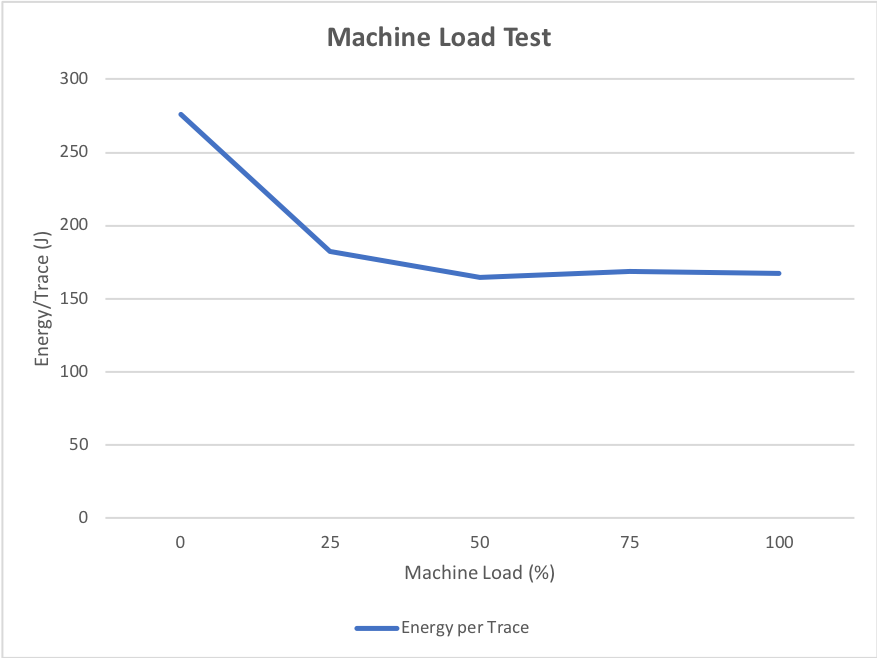
\includegraphics[width=0.75\textwidth,trim={2 2 2 2},clip]{Figures/validation-machineload}
\caption{Energy Allocation Under Different Host Load Conditions}
\label{figure:validation-machineload}
\end{figure}

As with some of our other testing, the results initially look somewhat counter-intuitive, but on further analysis are validation of consistent energy allocation by workload.

%  (Trace J at 25/50/75/100 prior load: 276, 183 [93], 164 [19], 169, 167)

The first point in the graph shows our workload running on an otherwise idle host and it is allocated quite a large amount of energy per trace (of 276J) because the host is relatively inefficient at lower levels of utilisation and there is no other workload on the host to allocate its energy to.

The second point in the graph shows a sharp reduction in energy per trace (to 183J), which is caused by the host's utilisation, which is now about 50\%, which is considerably more efficient than 25\% and the fact that the host's energy is being split between two roughly equivalent workloads.

The third point on the graph shows a further reduction in energy per trace (to 164J), which is a considerably smaller reduction than the previous step.  This is due to our share of the machine workload falling less significantly than in the previous step (from 49\% to 33\% whereas the previous step was from 96\% to 49\%).

The fourth point on the graph, at 75\% of other utilisation, actually goes up slightly (to 169J).  This is due to two factors.  Firstly, once again, our utilisation percentage drop decreases, this time from 33\% to 25\% (only 8\%) but secondly, the underlying machine becomes less efficient as utilisation moves beyond 75\% and so there is more energy to allocate between the different workload items.  This is an important insight for the application architect so that they consider the potentially non-linear energy consumption curve of the underlying host.

Finally at the fifth point on the graph, with 100\% other utilisation, our workload is competing with the existing workload to be scheduled for execution.  This results in our execution duration extending slightly (by 5\%), and our CPU utilisation percentage to drop slightly (to 23\%) with the result being a slight reduction in energy utilisation (to 167J).  This is the result of a relatively small increase in the host's energy utilisation (as it was already running close to 100\% utilisation at the previous sample) and there is now further workload to allocate the energy of the host across, so reducing our workload's allocation slightly.

This phase of testing was an interesting process because it illustrated the usefulness of investigating energy allocation using practical testing and a quantitative data-based allocation mechanism like Apollo.  It would be quite possible to make a simplistic assumption that fair energy allocation would keep falling linearly as load increased, but our tool can be used to provide a more sophisticated analysis that reveals how a complex interaction of a number of factors (including load, scenario length and host energy characteristics) can result in a correct allocation that is more complex.  This is a useful insight for the application architect as they investigate the energy characteristics of their application and this process allowed us to achieve validation goal 3.

\section{Validation Goal 4 - Validating CPU as a Resource Usage Proxy}

Validation goal V4 involves ensuring that CPU usage is a good proxy for overall resource usage of a piece of application software.

When we explained how the energy allocation process for an application's elements was to work, in \cref{chapter:monitoring}, part of the design of the allocation approach was to make the simplifying assumption that CPU utilisation is a good proxy for overall resource consumption (\sref{sec:utilisingresourceusage}).  This allowed  the approach to rely on CPU usage to allocate energy fairly.  While this assumption is based on previous research work \cite{bashroush2018_hardwarerefresh}, we were interested to test this assumption for ourselves by comparing IO activity with CPU utilisation.  

To test the assumption that CPU utilisation acts as a good proxy for IO activity, we wanted to find whether the two values correlated well during an application workload.  To test this we ran IO intensive workloads of varying known sizes and measured the CPU utilisation of each one.  The results of this exercise are shown in the line graph in \fref{figure:validation-traceenergydatasize}.  The x-axis of this graph shows the test scenarios, the left-hand y-axis is the amount of CPU measured for each scenario, the right-hand y-axis is the amount of energy allocated to each scenario.

\begin{figure}
\centering
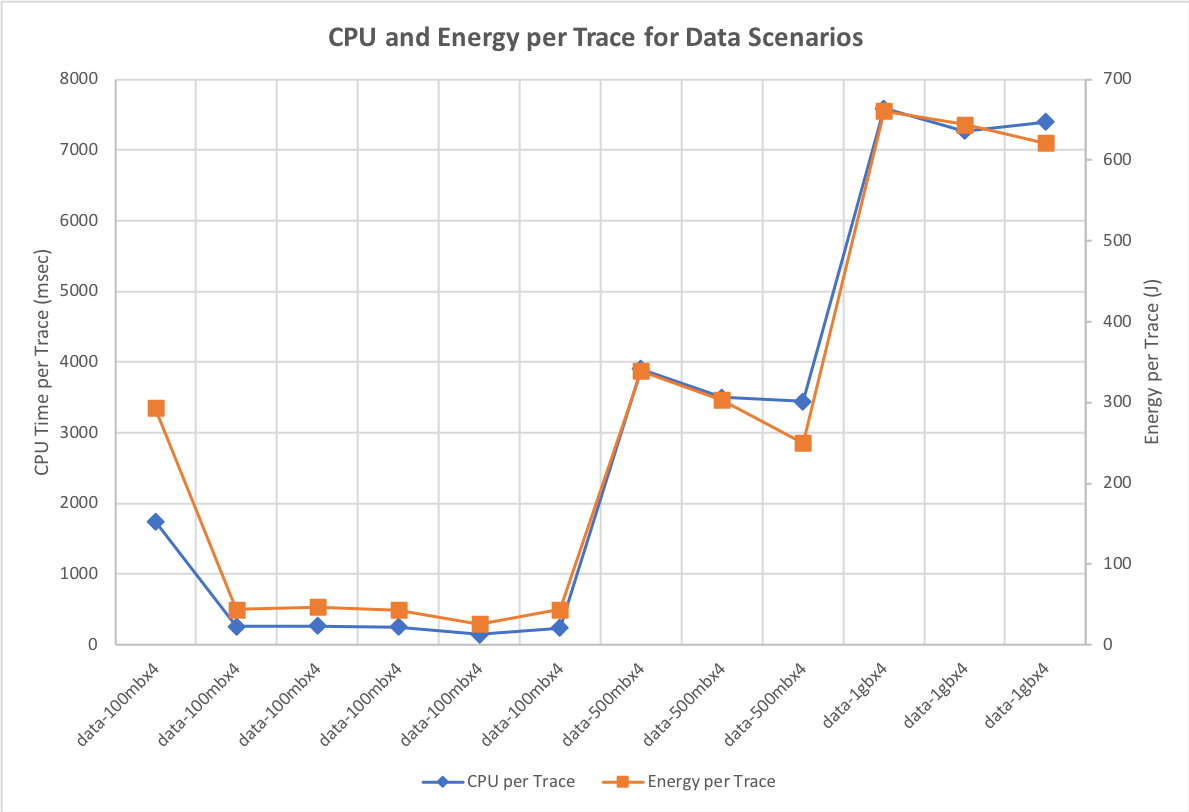
\includegraphics[width=0.75\textwidth,trim={2 2 2 2},clip]{Figures/validation-traceenergydatasize}
\caption{CPU Utilisation and Energy Allocation Scenarios}
\label{figure:validation-traceenergydatasize}
\end{figure}

The graph shows the results of running a number of data-intensive application scenarios, one group that called a service to write 100MB of data to file 4 times, one that called a service to write 500MB of data to file 4 times, and one that called a service to write 1GB of data to file 4 times.  Hence the total data written by the first group of scenarios was 400MB, the second group 2GB and the third 4GB.

When we plot the CPU usage and the Apollo energy allocation for the other test scenarios on the graph, we can clearly see that CPU usage is directly related to the amount of data written and the correlation coefficient between the values for data written and CPU utilised is 0.9965, indicating that CPU is a good proxy for the amount of data written by a process.

For completeness, we also plotted the data-size of each scenario compared to the energy allocated by Apollo to each, which is shown in \fref{figure:validation-energybydatasize}.  

\begin{figure}
\centering
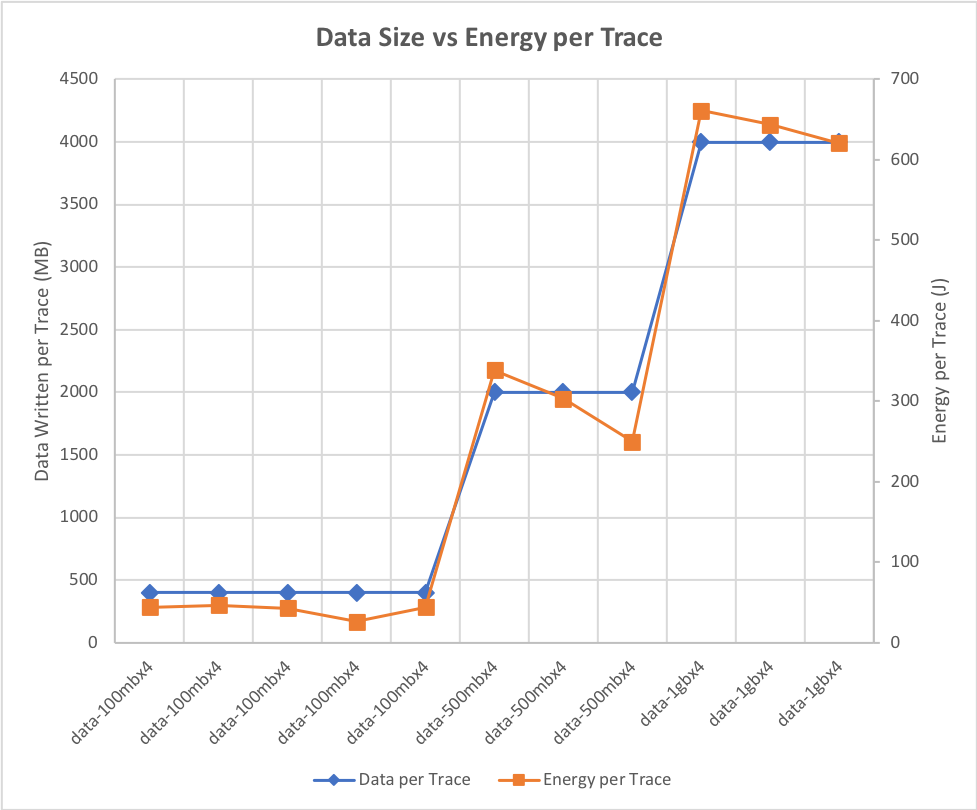
\includegraphics[width=0.75\textwidth,trim={2 2 2 2},clip]{Figures/validation-energybydatasize}
\caption{Energy Allocation by Data Size}
\label{figure:validation-energybydatasize}
\end{figure}

This graph looks similar to \fref{figure:validation-traceenergydatasize} but is illustrating a slightly different point in that while the x-axis (test scenarios) and right-hand y-axis (energy per trace) are the same, the left-hand y-axis shows the amount of data written by each scenario, rather than the CPU usage.  This can be seen in the flat horizontal sections of the graph for each type of scenario.  

The strong grouping of points around scenarios shows that this graph validates that the energy allocation for these data-intensive services correlates well with the amount of data each is writing, albeit with some variation in some test cases. When we calculated the correlation coefficient between energy allocation and data written, it was found to be 0.9967, again showing a very high degree of correlation between energy allocation and the amount of data written by the application elements within the scenario.

Finally, to provide some additional validation of the relationship of IO workload to CPU usage independent of Apollo, we performed some detailed manual tests, calling the microservice directly and measuring CPU usage before and after service invocations for different amounts of IO.  The CPU usage was read directly from the \texttt{/proc/PID/stat} operating system statistics.

\begin{figure}
\centering
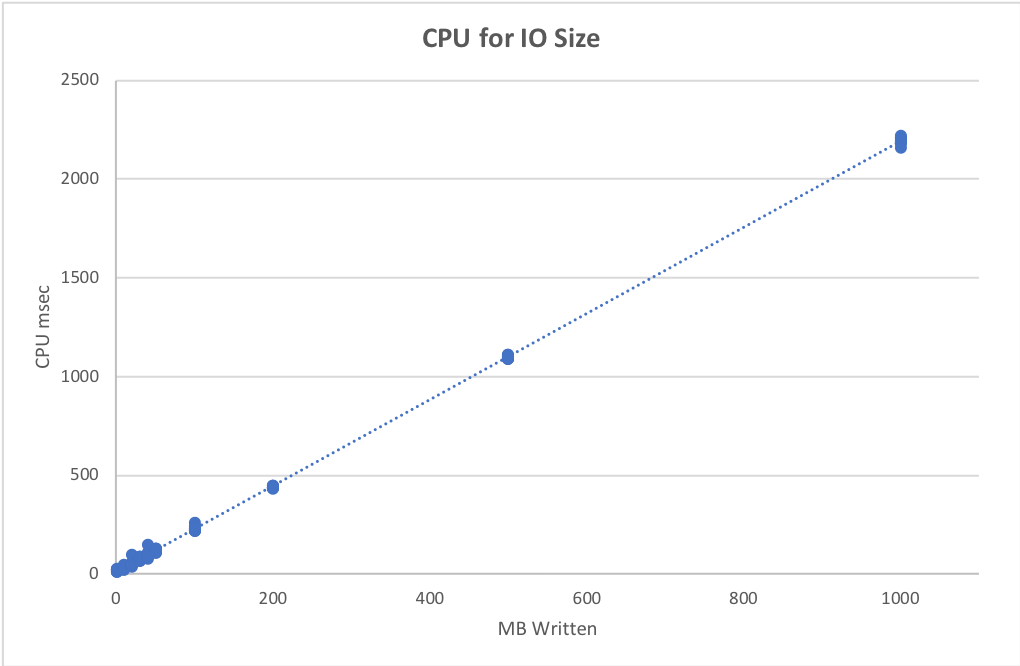
\includegraphics[width=0.75\textwidth,trim={3 2 2 2},clip]{Figures/validation-cpubydatasize}
\caption{Energy Allocation by Data Size}
\label{figure:validation-cpubydatasize}
\end{figure}

The result of these manual tests is shown in the scatter plot and trend line shown in \fref{figure:validation-cpubydatasize}.  The y-axis shows the amount of CPU used by the service per request, the x-axis the amount of data written by each request and each point on the graph is a single service invocation.  As the graph shows there is a strong correlation between the amount of data written and the CPU consumed for the service call and when we calculated the correlation coefficient, it was found to be 0.9998, confirming this finding.  By using the difference in data size and CPU utilisation between samples, we were also able to calculate that 1 MB of file IO write activity appears to require approximately 2ms of CPU time on our test machine.

The combination of these test results shows that we were correct in our assumption that CPU is a good proxy for other resource utilisation by a process and achieves validation goal 4.

\section{Conclusions}
\label{sec:energy-conclusions}

In order to validate our proof-of-concept implementation of the Apollo Energy Allocator system, we identified four validation goals that we needed to achieve.

\begin{itemize}
	\item \textit{Validation Goal 1 - Calculation Correctness} which involves running the calculator in a realistic, but reasonably simple, scenario, under controlled conditions and replicating its calculation process as independently as possible.
	\item \textit{Validation Goal 2 - Calculation Consistency} which involves running a number of test scenarios with different characteristics and comparing the energy allocation results provided by Apollo, to ensure consistency between different types of scenario.
	\item \textit{Validation Goal 3 - Energy Allocation Algorithm} which requires us to run identical scenarios in situations with different amounts of controlled competing workload on the host machine(s) to allow us to validate that Apollo allocates energy fairly across these workload profiles.
	\item \textit{Validation Goal 4 - CPU Usage as a Proxy for Resource Usage} which confirms that the previous research result that suggested that CPU usage was a valid proxy measure for overall resource utilisation, and in particular for disk IO activity.
\end{itemize}

As stated earlier, our aim was to achieve consistency of results to within 5\% tolerance as practical experience has taught us that results within this tolerance level are effectively equal in performance and resource usage testing, given the number of dynamic factors outside our control.

The testing presented in this chapter has specifically addressed each of these aspects of validation.

We performed a manual data collection and calculation exercise in order to validate goal 1, \textit{Calculation Correctness}, as described in \sref{sec:validatingcalculation}.  The result of this exercise, based on independent resource utilisation data sources, separate from the data used by Apollo, was an energy allocation value within 4\%  of the value calculated by Apollo.

We then investigated goal 2, \textit{Calculation Consistency}, by performing a series of CPU intensive workload tests, as described in \sref{section:validatingconsistency}, that ran controlled application workloads for different levels of resource consumption, in order to confirm that Apollo allocated energy correctly and consistently for all of the test cases.  These test cases proved that there was a very high degree of correlation between our different levels of application workload and the energy allocation that each received, so proving that the energy allocation was consistent across varying workload.

The next step was to validate goal 3, \textit{Energy Allocation Algorithm}, as described in \sref{section:validatingallocation}, by running controlled test workloads on host machines that had carefully controlled competing workload running on them already. These tests proved that when competing workload was present on a host machine, energy was allocated correctly between our test workload and the competing workload and was well within the 5\% level of consistency that we were aiming for.

Finally, we investigated whether validation goal 4, \textit{CPU Usage as a Proxy for Resource Usage}, was correct for an application trace.  We were aware of previous research results suggesting that this was the case, but we decided to investigate it empirically in our specific situation too.  We focused on file IO during this part of the investigation and ran a number of tests to investigate its relationship to CPU usage.  These tests confirmed that CPU usage is a very good proxy for file IO usage, with a correlation coefficient greater than 0.9 for the two values.

In summary, we have investigated four different aspects of the correctness and utility of the Apollo Energy Allocation System's proof-of-concept implementation of our energy allocation approach for application-level energy monitoring.  All four of the testing exercises confirmed a different aspect of the correctness of the implementation.  Therefore, we conclude that the proof-of-concept implementation is sufficiently consistent and correct to validate the application energy allocation approach that we propose.

